\section{Tactical combat - Battlescape}

The goal of every tactical combat is simple: kill all the aliens with as few civilian and squad losses as possible. In order to achieve this you will have to find a good balance between caution and speed. You don't want to watch all innocents die like flies just because your soldiers are afraid of the enemy.  If you cannot succeed in tactical combat, you will never succeed in the game.

During the course of gameplay, you will see a wide range of settings and environments, but no matter how bad things may look, there are some powerful tools at hand. If you have some experience with (turn-based) tactical combat games you should find some familiar elements. Nevertheless, you should take a short overview over the interface so as not to miss any important features.

To change the view within battlescape you may use either cursor or the \keybinding{WASD} keys. Please be aware that its also possible to change the pitch of the camera -- \keybinding{R} and \keybinding{F} by default.

There are currently two alternative interfaces available, offering identical functions with a different look. You may switch between them as often as you want, using options $\hookrightarrow$ game. While the first one is heavily inspired by the classic HUD, the second one (althud) tries to utilise modern techniques to achieve a cleaner look.

\subsection{Buttons - HUD}
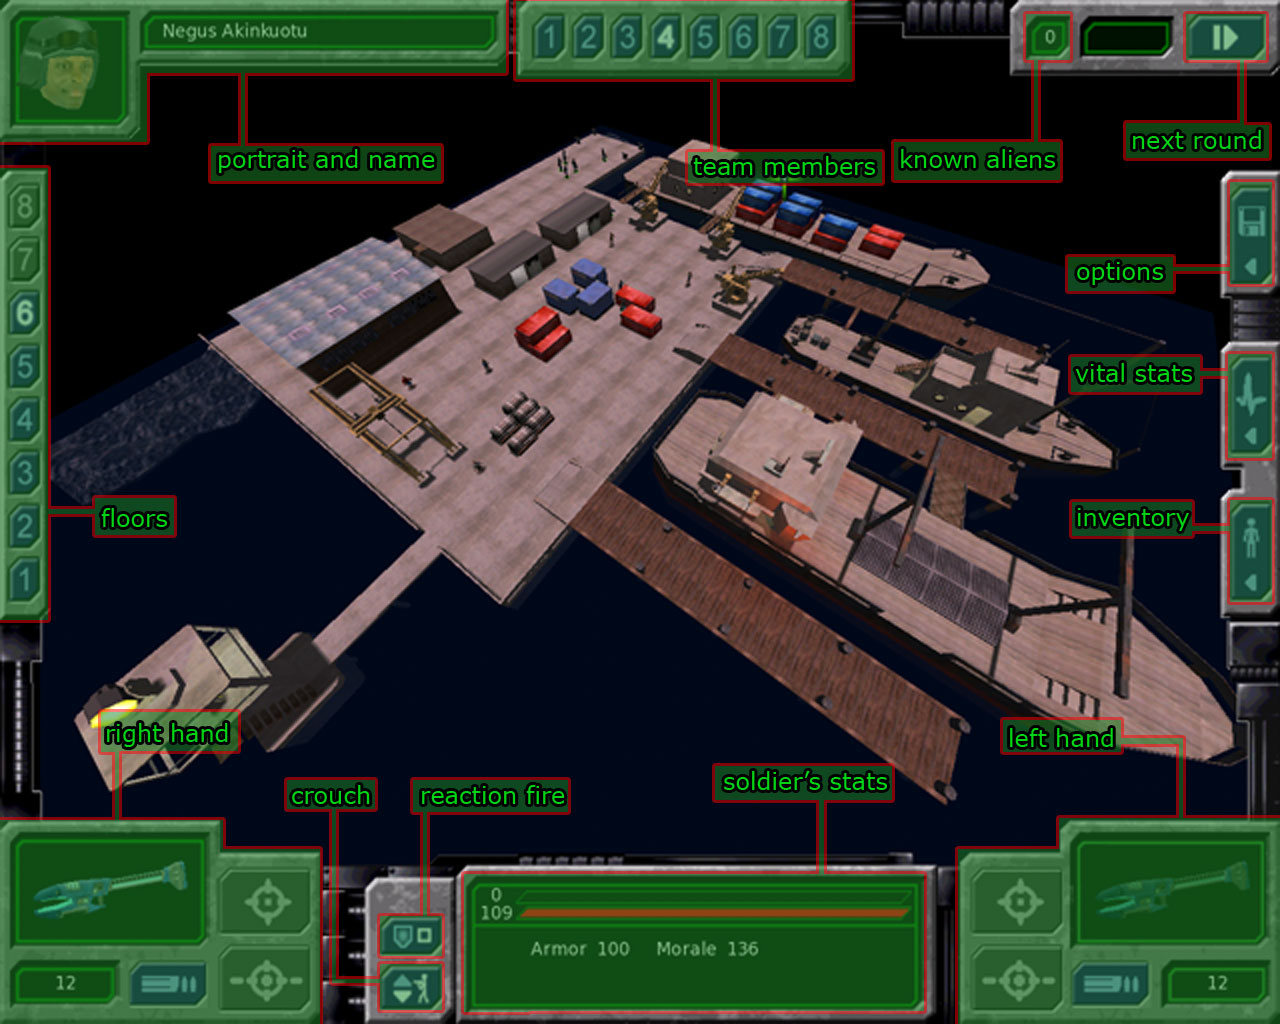
\includegraphics[width=\textwidth]{images/HUD_final.jpg}
\subsubsection{Floors}
Here you can change the ``floor'' shown in the tactical view. Besides its obvious use in helping you to move your soldiers between different levels, it's also used to get an general overview. You should always switch between all levels at the beginning of each mission so you won't miss the ``hidden'' cellar or rooftop.

\subsubsection{Portrait and name}
This is more for aesthetic reasons, and does not currently perform any function.

\subsubsection{Team members}
Use this to switch between your soldiers. Alternatively use keybindings: \keybinding{1} to \keybinding{8}, or you can also just left-click on their model. If one of your soldiers is killed, his button will turn grey and become non-functional.

\subsubsection{Known aliens}
This indicates the number of aliens all your squad member have discovered. You may switch through all of them by clicking this button.

\subsubsection{Next round}
This immediately proceeds to the next game turn.

\subsubsection{Options}
Opens the \emph{Options} menu where you may alter several video and sound settings, as well as abort or retry the current mission. You may not save an ongoing mission. If you abort the current mission, all your soldiers will be lost.

\subsubsection{Vital stats}
Here you will find more detailed information about health, morale, and psi-power of your individual soldiers.

\subsubsection{Inventory}
Opens the inventory of the selected soldier. This is where you can change weapons, pick up and drop items, or just take a look at your great heroes.

\subsubsection{Soldiers stats}
This is a summary of all general information you need to use your soldier. It is context-sensitive, and hopefully self-explanatory.  Here you will find information like remaining health and TUs (dealt with in the following section), how many TUs your currently selected shooting-mode will consume, current armour, and morale.

\subsubsection{Reaction fire}
Reaction fire will be dealt with in a later section, so for now you should just remember that this is where you turn it on and off.

\subsubsection{Crouch}
Clicking this will cause your soldier to crouch or stand up.  Crouching reduces the danger of being hit by enemy fire, but causes movement to cost 1 extra TU per square.

\subsubsection{Right/left-hand}
While all soldiers are right-handed, they can still wield a weapon in each hand. If you have a two-handed item/weapon equipped the left-hand field will be inactive. Please take a look at the following image.\\
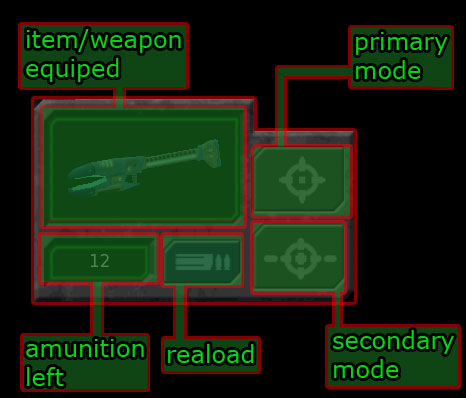
\includegraphics[width=6cm]{images/HUD_detail_final.jpg}
%as float ?!
%transparent background ?! ->going to be re-worked soon

\subsubsection{Item/weapon}
Gives a picture of the currently equipped item/weapon. This turns red if you can't use the weapon, if you don't know the technology or are out of ammunition for it.

\subsubsection{Primary and secondary item modes}
The primary mode for a weapon is usually a faster but less accurate or powerful shot. Weapons include more details in their item description.  The secondary mode for a weapon generally includes a more powerful or accurate shot, which consumes more TUs when activated.  Some items only support one usage mode.

\subsubsection{Reload}
If your soldier has remaining ammunition in his inventory, this will cause him to reload as fully as possible. Reloading always uses TUs, the amount of which varies according to the weapon type.

\subparagraph{Remaining ammunition}
Shows the ammunition left in your weapon. Some shooting modes use more than one unit of ammunition; for instance, a burst from an automatic weapon.

\subsection{Buttons - altHUD}

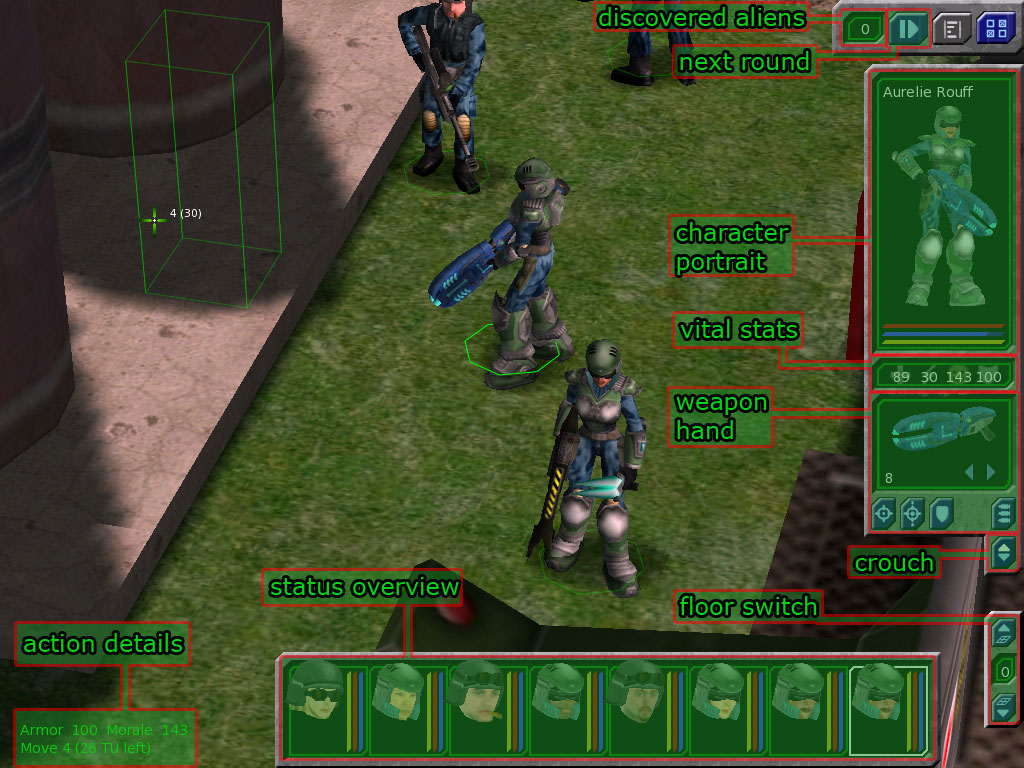
\includegraphics[width=\textwidth]{images/altHUD_final.jpg}\\

All the buttons in the altHUD perform exactly the same functions as in the primary HUD, so please refer to that section for details.
